\documentclass[12pt,fleqn]{article}
%\usepackage{fullpage}
\author{Bernie, Mogire}
\title{Additive Manufacturing}
\usepackage{a4}
\usepackage{graphicx}
\usepackage{subfig}
\usepackage{bookmark}
\usepackage{psfrag}
\usepackage{amsmath}                     % \boldsymbol{#1}
\usepackage{amssymb}
%\usepackage{hangcaption}
%\usepackage{Styles/pstricks}
%\usepackage{Styles/pst-node}
\usepackage{Styles/fancyheadings}
\usepackage{tocloft}
%-----Tex width---------------------------------
\textwidth 16cm
\textwidth 16cm

%-----Line spacing-------------------------------
\renewcommand{\baselinestretch}{1.5}     % 1,1-zeilig

%---------Add dots in TOC-----------------------
\renewcommand{\cftsecleader}{\cftdotfill{\cftdotsep}}

%------Paragraph indention-------------------------------
\setlength{\parskip}{1.5ex plus0.5ex minus0.5ex}

%-----Prevent indent----------------------
\setlength{\parindent}{0em}

%-----Richtiger Abstand fur Einheiten-------------
\def\Unit{\hspace{0.25em}}

%-----Definition of the header--------------------
\pagestyle{fancyplain}
\renewcommand{\sectionmark}[1]{\markboth{Chapter~\thesection.~#1}{#1}}
\renewcommand{\subsectionmark}[1]{\markright{\thesubsection\ #1}}
\rhead[\fancyplain{}{\leftmark}]%
{\fancyplain{\thepage}{\thepage}} \cfoot{} \plainheadrulewidth
0.4pt
%% Otherwise: Overfull \vbox-Warning against fancyheadings-pacakage
%%  idea of: nic@minster.york.ac.uk (Nick Cropper)
\makeatletter
\ifcase \@ptsize \relax % 10pt
  \addtolength{\headheight}{1\p@}
\or % 11pt
  \addtolength{\headheight}{2\p@}
\or % 12pt
  \addtolength{\headheight}{3\p@}
\fi \makeatother

%-----Equations / Figures / Tables numbering according to \ sections
\makeatletter
\renewcommand\theequation{\thesection.\arabic{equation}}
\renewcommand\thefigure{\thesection.\arabic{figure}}
\renewcommand\thetable{\thesection.\arabic{table}}
\@addtoreset{equation}{section} \@addtoreset{figure}{section}
\@addtoreset{table}{section} \makeatother

%-----Useful abbreviations----------------------
\newcommand{\mr}{\mathrm}
\newcommand{\bs}[1]{\mbox{$\boldsymbol{#1}$}}
\newcommand{\degree}[1]{\mbox{$#1^\circ$}}

%\renewcommand{\figurename}{Bild}

%------Bibliography style-----------------------
\bibliographystyle{IEEEtran}

%-----Aufzaehlunstiefe im Literaturverzeichnis---------------
\setcounter{tocdepth}{3}

\begin{document}
\pagenumbering{Roman}
\begin{titlepage}
  \begin{center}
      \vspace*{-4.0cm}
    \begin{figure}[!h]
\centering

\includegraphics[width=0.3 \linewidth] {Figures/JKUAT_logo}
%\caption{}
\label{fig:jomologo}
\end{figure}
   \large{Jomo Kenyatta University of Agriculture and Technology}\\
    \large{College of Engineering and Technology}\\
    \large{School of Mechanical, Materials, and Manufacturing Engineering}\\
   \large{Department of Mechatronic Engineering}\\

    ------------------------------------------------------------------------------------------------\\[1.0cm]
    \LARGE{\textbf{EMT 2540: PRACTICAL REPORT I}}\\[0.6cm]
    \LARGE{\textbf{ADDITIVE MANUFACTURING
            }}\\[1.5cm]
    %\large{by}\\[0.6cm

    \vspace{0.5cm}
    \large{\textbf{Bernie Kiplelgo Cheruiyot (ENM221-0054/2017)
            }}\\
     \large{\textbf{Mogire Earl Spencer (ENM221-0074/2017)
            }}\\[1.0cm]
%     \large{\textbf{Supervisors}}\\
%    \large{Dr.-Ing.~Jackson G. Njiri}\\
%    \large{Prof. George N. Nyakoe}\\
%    \large{\ldots}    \\[0.2cm]\vfill
    \large{\small{\today}}\\
    ------------------------------------------------------------------------------------------------\\[1.5cm]
  \end{center}
\end{titlepage}
%
%\pagenumbering{gobble}% Remove page numbers (and reset to 1)

%\addcontentsline{toc}{section}{Declaration}
\section*{Declaration}


We hereby declare that the work contained in this report is original; researched and documented by the undersigned students. It has not been used or presented elsewhere in any form for award of any academic qualification or otherwise. Any material obtained from other parties have been duly acknowledged. We have ensured that no violation of copyright or intellectual property rights have been committed.
\begin{enumerate}
	\item Theodore Kamau\vspace*{.2cm}\\
	Signature\ldots\ldots\ldots\ldots\ldots\ldots\ldots\ldots\ldots\ldots Date\ldots\ldots\ldots\ldots\ldots\ldots\ldots\ldots\ldots\ldots
	\item Lisa Kimondo\vspace*{.2cm}\\
	Signature\ldots\ldots\ldots\ldots\ldots\ldots\ldots\ldots\ldots\ldots Date\ldots\ldots\ldots\ldots\ldots\ldots\ldots\ldots\ldots\ldots
\end{enumerate}

\vspace*{.5cm}
Approved by supervisors:
\begin{enumerate}
	\item Dr.-Ing. Jackson G. Njiri\vspace*{.2cm}\\
	Signature\ldots\ldots\ldots\ldots\ldots\ldots\ldots\ldots\ldots\ldots Date\ldots\ldots\ldots\ldots\ldots\ldots\ldots\ldots\ldots\ldots
	\item Prof. George N. Nyakoe\vspace*{.2cm}\\
	Signature\ldots\ldots\ldots\ldots\ldots\ldots\ldots\ldots\ldots\ldots Date\ldots\ldots\ldots\ldots\ldots\ldots\ldots\ldots\ldots\ldots
	\item Ms. Lucy W. Kariuki\vspace*{.2cm}\\
	Signature\ldots\ldots\ldots\ldots\ldots\ldots\ldots\ldots\ldots\ldots Date\ldots\ldots\ldots\ldots\ldots\ldots\ldots\ldots\ldots\ldots
\end{enumerate}



%\clearpage
\addcontentsline{toc}{section}{Table of Contents}
\tableofcontents
\clearpage
\addcontentsline{toc}{section}{List of Figures}

\let\oldnumberline\numberline%
\renewcommand{\numberline}{\figurename~\oldnumberline}%
\lhead{\textit{LIST OF FIGURES}}
\listoffigures
\clearpage
%\lhead{\textit{LIST OF TABLES}}
%\renewcommand{\numberline}{\tablename~\oldnumberline}%
%\addcontentsline{toc}{section}{List of Tables}
%\listoftables
%\newpage
%\clearpage
%\addcontentsline{toc}{section}{List of Abbreviations}
%\paragraph{Nomenclature}
\begin{itemize}
\item 2D - Two dimensional
\item 3D - Three dimensional
\item AM - Additive Manufacturing
\item CAD - Computer Aided Design
\item CAE - Computer Aided Engineering
\item CT - Computerized Tomography
\item FDM - Fused Deposition Modeling
\item RE - Reverse Engineering
\item STL - Standard Triangle Language/Standard Tessellation Language
\end{itemize}
\pagebreak
\clearpage
\newpage
\clearpage

\clearpage
\pagenumbering{arabic}
  \chapter{Introduction}
\lhead{\leftmark}
\label{sec:introduction}
\section{Additive Manufacturing}
Additive Manufacturing (AM) is a manufacturing technology that uses the additive approach in the fabrication of parts. AM significantly
simplifies the process of producing complex 3D objects directly from CAD data .

3D Printing has become the most commonly used wording to describe AM technologies. This term alludes to the use of a 2D process (printing) and extending them into the third dimension. Significant improvements in accuracy and material properties have seen 3D printing
technology become useful in other applications other than prototyping. These applications are: testing, tooling, manufacturing, etc. 

3D printing is a rapid and seamless process. It also reduces the amount of resources and processes required significantly. With the addition of some supporting technologies like silicone-rubber
molding, drills, polishers, grinders, etc. AM can be possible to manufacture a vast
range of different parts with different characteristics. Workshops which adopt AM
technology can be much cleaner, more streamlined, and more versatile than before.

\section{Objectives}
\begin{enumerate}
\item To design a CAD model of a complex 3D part.
\item To fabricate the complex 3D part using an Additive Manufacturing technique (3D Printing)
\end{enumerate}

  \clearpage
  \chapter{Literature Review}
\lhead{\leftmark}
\label{sec:review}
%
\section{Additive Manufacturing}
Additive manufacturing, referred to in short as AM, is the basic principle of generating a model using a three-dimensional Computer-Aided Design (3D CAD)
system and fabricating it directly without the need for process planning. In contrast to other manufacturing processes, AM needs only some basic dimensional details and a small amount of knowledge on how the AM machine works and the materials that are used to build the part\cite{edgar2015additive}.

The basic working principle for AM works is that parts are made by adding material in layers, each layer being a thin cross-section of the part derived from the original CAD data. Layer thickness will affect the final output: the thinner each layer is, the closer the final part will be to the original\cite{classnotes}.

Additive Manufacturing, commonly referred as 3D printing is a computer-based technology. Like many  other manufacturing
technologies, improvements in computing power and reduction in mass storage
costs paved the way for processing the large amounts of data typical of modern 3D
Computer-Aided Design (CAD) models within reasonable time frames. AM takes full advantage of many of the important features of computer technology,
both directly (in the AM machines themselves) and indirectly (within the supporting technology). 

\section{Technologies Associated with AM}
The most common input method for AM technology is to accept a file converted
into the STL file format originally built within a conventional 3D CAD system.
There are, however, other ways in which the STL files can be generated and other
technologies that can be used in conjunction with AM technology. These are\cite{edgar2015additive}:

\subsection{Reverse Engineering Technology}
Reverse Engineering (RE) is the process of
capturing geometric data from another object, commonly referred to as 3D scanning. These data is initially available “point cloud” form i.e. an unconnected set of points representing the object surfaces. These points need to be connected together
using RE software like Artec, which may also be used to combine point clouds from different scans and to perform other functions like hole-filling and
smoothing.

Engineered objects are scanned using laser-scanning or touch probe technology. Objects that have complex internal features or anatomical
models may make use of Computerized Tomography (CT).

\subsection{Computer Aided Engineering}
Direct Digital Manufacture, where AM can be used to directly produce
final products, requires Computer Aided Engineering (CAE) tools to evaluate how these parts
would perform prior to AM. This ensures that we can build products right the first time as a
form of Design for Additive Manufacturing (D for AM).

\subsection{Heptic Based CAD}
CAD modeling systems work
in a similar way to Freeform modeling systems to
provide a design environment that is more intuitive than other standard CAD
systems. They often use a robotic haptic feedback device called the Phantom to provide force feedback relating to the virtual modeling environment. An object can
be seen on-screen, but also felt in 3D space using the Phantom. The modeling
environment includes what is known as Virtual Clay that deforms under force
applied using the haptic cursor. This provides a mechanism for direct interaction
with the modeling material, much like how a sculptor interacts with actual clay. Basically, this is CAD for non-engineers for non-engineering applcations.

\section{Classification of AM Processes}
\begin{enumerate}
\item Vat photo-polymerization - processes that utilize a liquid photo polymer that is
contained in a vat and processed by selectively delivering energy to cure specific
regions of a part cross-section.
\item Material extrusion - processes that deposit a material by extruding it through a
nozzle, typically while scanning the nozzle in a pattern that produces a part
cross-section.
\item Material jetting: ink-jet printing processes.
\item Binder jetting - processes where a binder is printed into a powder bed in order to
form part cross-sections.
\item Sheet lamination: processes that deposit a layer of material at a time, where the
material is in sheet form.
\item Directed energy deposition - processes that simultaneously deposit a material
(usually powder or wire) and provide energy to process that material through a
single deposition device.
\item Fused Deposition Modeling (FDM).
\end{enumerate}
FDM uses a
heating chamber to liquefy polymer that is fed into the system as a filament. The filament is pushed into the chamber by a tractor wheel arrangement and it is this
pushing that generates the extrusion pressure\cite{classnotes}.

  \clearpage
    \section{Methodology}
\lhead{\leftmark}
The equipment needed and procedures undertaken to carry out 3D printing are described in the following sections. The experiment was done at iPIC (Rapid Prototyping Lab) in JKUAT.
\subsection{Equipment}
\begin{enumerate}
\item 3D Scanning hardware and software (Artec3D, Artec Spider, Artec Studio.)
\item Workpiece shown in Figure \ref{fig:3dscan}
\item 3D Printing hardware and software (Tiertime Up! Mini)
\end{enumerate}
\begin{center}
	\begin{figure}[h!]
	\centering
	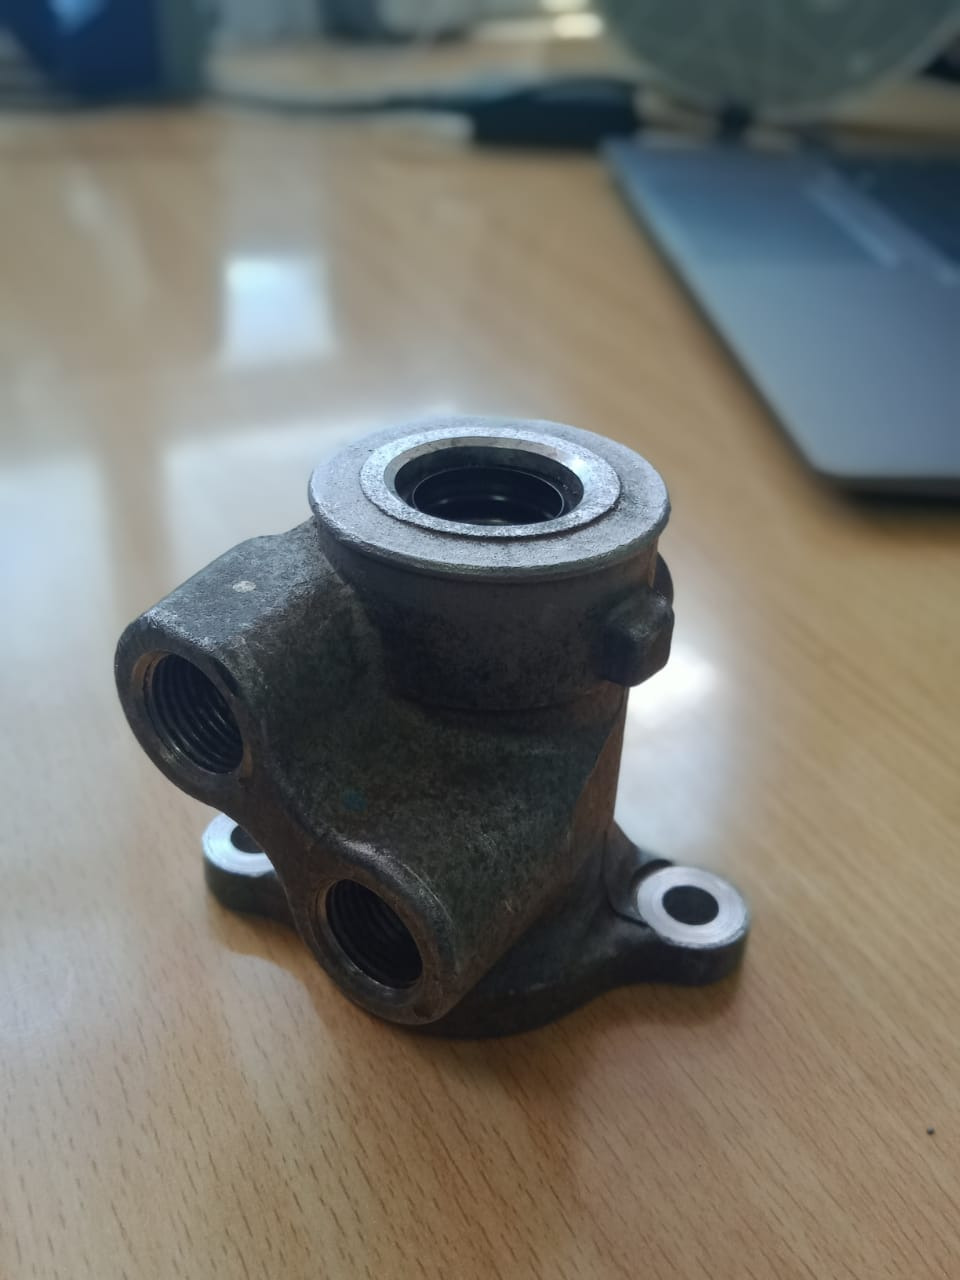
\includegraphics[width=0.4\linewidth]{Figures/Figure}
	\caption{Complex Workpiece}
	\label{fig:3dscan}
	\end{figure}
\end{center}
\newpage
\subsection{Procedure}
The 3D scanning hardware and software were set up and the workpiece placed on the turntable for scanning. Figure \ref{fig:scanning} shows the workpiece being scanned.\\
Several scans were performed and the final 3D model was obtained. Some post-processing was performed on the 3D Scan data before processing it into a 3D Model. Some of these procedures are:
\begin{enumerate}
	\item Aligning the multiple scans using various coincident points and axes on each scan.
	\item Denoising - removing noisy areas from the scan.
	\item Trimming unwanted parts from the scan.
	\item Making adjustments to distorted geometry.
\end{enumerate} 
\begin{center}
 	\begin{figure}[h!]
 	\centering
 	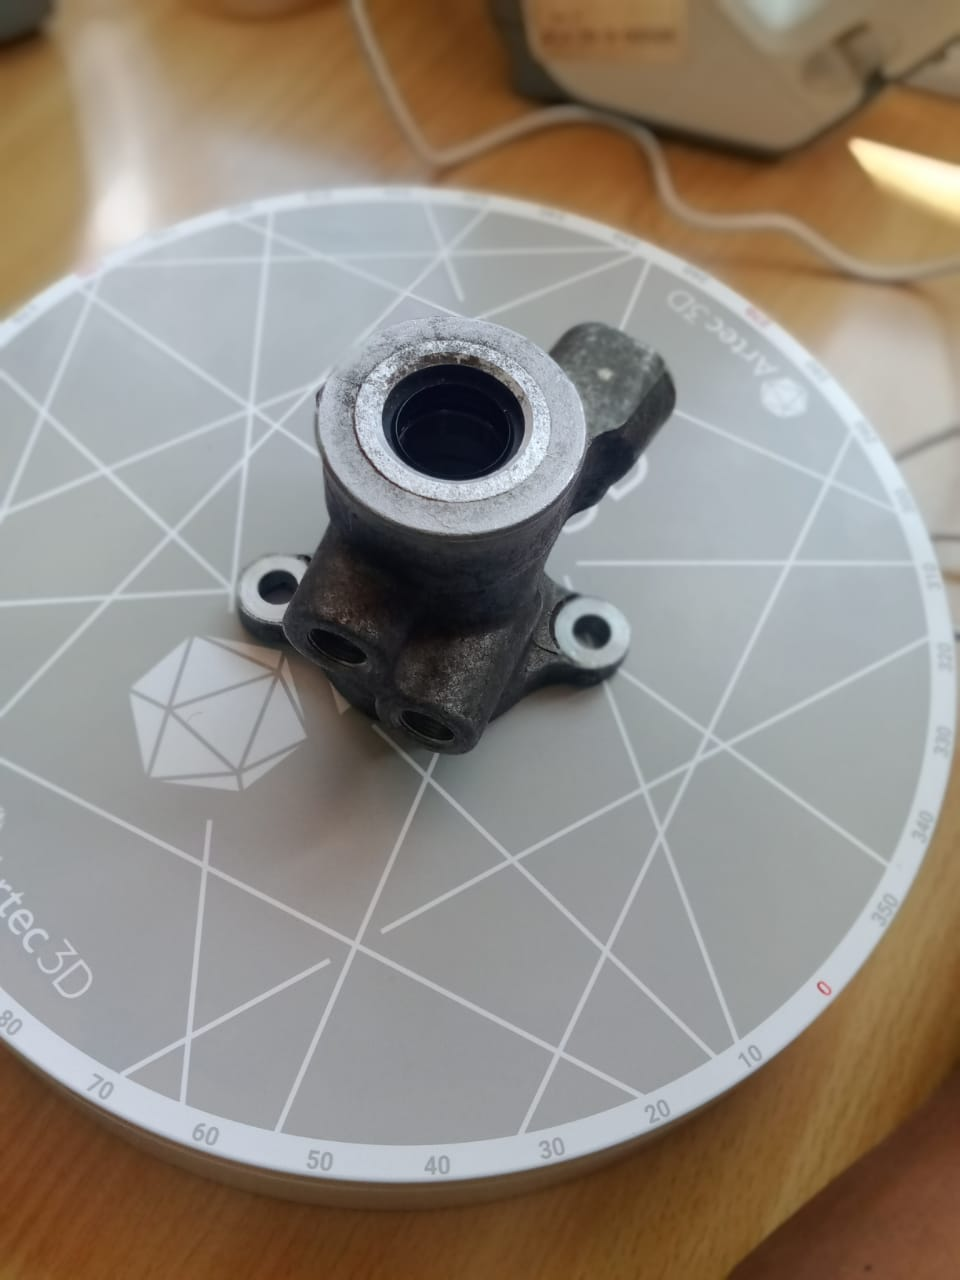
\includegraphics[width=0.4\linewidth]{Figures/Figure 2}
 	\caption[Scanning]{Workpiece being scanned}
 	\label{fig:scanning}
 	\end{figure}
 \end{center}
In this practical exercise, FDM was used to come up with a 3D object.

  \clearpage
 \chapter{Results}
  \clearpage
    \section{Discussion}
\subsection{3D Scanning}
The reverse engineering process is able to replicate an existing object with a great degree of dimensional accuracy and identical geometry. This eliminates the need for accurate measurements and complicated 3D CAD techniques to obtain a 3D Model of an existing product.\\
While the model obtained is quite close to the original, there are still some inaccuracies in the 3D scan. Some of these are:
\begin{enumerate}
	\item Distorted screw threads.
	\item Blocked holes.
	\item Inaccurate internal geometry.
	\item Creation of non-existent geometry.
\end{enumerate}
Some of these inaccuracies in the 3D Scan can be minimised by using proper technique and setting up a good scanning environment. Some of the ways to improve the quality of a scan are:
\begin{enumerate}
	\item Ensuring the scanning area is well lit
	\item Scanning dark or non-reflective objects. A thin coating such as fine charcoal dust can be applied to the object to improve scan results.
	\item Carrying out several scans to capture geometries on the opposite side of the scanner.
	\item Using a turntable to rotate the specimen at a constant speed, as well as synchronising the angular speed with the scanner's polling rate.
\end{enumerate}
  \clearpage
%  \section{Appendices}
  \clearpage
%----  Bibliography  ----------------------------------------
\markright{References}                               % Erzeugt Kopfzeile
\addcontentsline{toc}{section}{References}            % Literaturverzeichnis ins Inhaltsverzeichnis
\bibliographystyle{Bib/IEEEtran}
\bibliography{Bib/References}                         % BIBTeX
\nocite{Lun01} 

                                     % Falls etwas in die Literaturliste soll, was nicht Referenziert wird
\end{document}